\chapter{Methodology}
\label{ch:methodology}
The overall process of developing the WebArgo platform presented in this work consited of the following steps:
\begin{enumerate}
  \item Theoretical design of the platforms Architecture
  \item Development of a Proof of Concept prototype
  \item Development process from the prototype to the WebArgo platform
  \begin{itemize}
    \item Implementation of \acs{API} and web interface
    \item Usage of generic job and task entities to support any kind of custom job
    \item Add WebAssembly Support for multiple programming languages
    \item Implement support for various output datatypes (primitiv datatypes, lists, files as binary)
  \end{itemize}
  \item Deployment of the web application
  \begin{itemize}
    \item Orchestrate all components of the WebArgo platform with Docker Compose \cite{conclusion:docker}
    \item Host the project on a cloud services (\emph{openstack} from h\_da)
    \item Implement user entity with specific user roles to enable security
    \item Implement security measures through authentication \& authorization
  \end{itemize}
  \item Enhance robustness of the platform
  \begin{itemize}
    \item Implement system recovery measures and persistence of critical data
    \item Adjust scheduling algorithm to ensure the completion of jobs, even when workers are unreliable
    \item Eliminate bugs through testing the application
  \end{itemize}
  \item Implement the visualization of the Mandelbrot set in multiple languages as the benchmark job
  \item Evaluation of the platform through multiple experiments 
\end{enumerate}
The following content of this chapter enumerates and describes all the technologies, frameworks, and tools utilized in the development of the volunteer computing platform, along with the reasoning for their selection. Each section provides a detailed explanation of these components, establishing a foundation for the following \autoref{ch:implementation} which focuses on the implementation. Additionally, all entities are listed and described in \autoref{sec:methodology:entities} to define all specific terms used in the subsequent chapters.

\section{Entities}
\label{sec:methodology:entities}
This section describes all entities and establishes the terms used to describe the processes in this work.

\subsection{Job}
\label{subsec:methodology:entities:job}
The job entity represents a problem to be processed or solved using the platform. The platform is designed to handle multiple jobs while each job is a unique object. The State of a job can have one of the following values:
\begin{itemize}
  \item PENDING
  \item ACTIVE
  \item RUNNING
  \item STOPPED
  \item DONE
\end{itemize}
\begin{figure}[htbp]
  \centering
  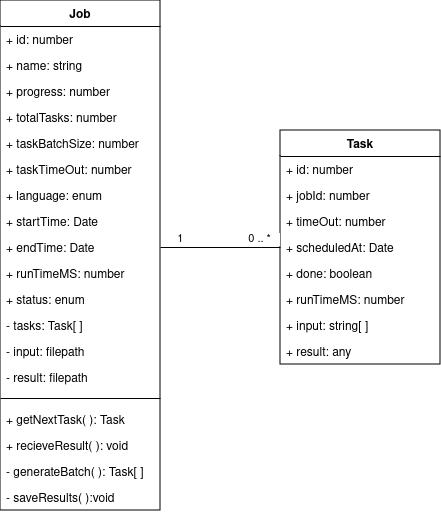
\includegraphics[width=0.75\textwidth]{gfx/figures/Job-Task.png}
  \caption{\acs{UML} Class Diagram: Job \& Task}
  \label{fig:methodology:job-task}
\end{figure}
\autoref{fig:methodology:job-task} illustrates the \ac{UML} class diagram for the job entity on the left side, lisitng all important attributes and methods of a job. The language attribute defines the programming langugae of the source code that has been compiled to a WebAssembly binary file.

\subsection{Task}
\label{subsec:methodology:entities:task}
Each job is divided into multiple equally sized tasks. These tasks are distributed to the worker nodes of the platform. Tasks are unique objects, each holding the specific input parameters that describe the particular portion of the job to which the task is assigned. \autoref{fig:methodology:job-task} displays the \ac{UML} class diagram for the task entity on the right side. The relationship between the job and task entities is defined as One-to-Many, meaning a job can consist of multiple tasks, but each task is always assigned to a single job.

\subsubsection{Batch}
\label{ssubsec:methodology:entities:task:batch}
A batch is defined to be a subset of tasks, wich are all assigned to the same job.

\subsection{Client}
\label{subsec:methodology:entities:client}
\begin{figure}[htbp]
  \centering
  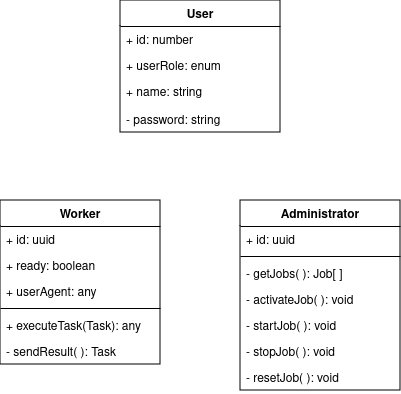
\includegraphics[width=0.75\textwidth]{gfx/figures/Client.png}
  \caption{\acs{UML} Class Diagram: User - Worker \& Administrator}
  \label{fig:methodology:client}
\end{figure}
~\\
A client represents a node that accesses the platform. The actions a client can perform are determined by the user role assigned to its user. This user role can either have the value \emph{User} for limited access or \emph{Admin} for full access to all features. \autoref{fig:methodology:client} displays the \ac{UML} class diagram for the user entity at the top of the illustration.

\subsubsection{Worker}
\label{ssubsec:methodology:entities:client:worker}
Workers are clients that voluntarily donate their computing power to support an active job. Therfore they receive tasks from the current batch sent by the server (\autoref{subsec:methodology:entities:Server}), compute these tasks, and return the corresponding results back to the server. \autoref{fig:methodology:client} presents the \ac{UML} class diagram of the worker entity on the left side, listing all relevant attributes and methods. As workers connect to the server via web browsers, the browser's user agent is utilized to individually characterize each worker. This so called browser user agent can be accessed inside the clients browser environment and provides information about the client's hardware resources and operating system.

\subsubsection{Administrator}
\label{ssubsec:methodology:entities:client:admin}
An administrator client can perform the same actions as a worker, but also has additional capabilities. Only administrators have the ability to set or change the state of jobs and to oversee the progress of all jobs. \autoref{fig:methodology:client} illustrates the \ac{UML} class diagram of the administrator entity on the right side.

\subsection{Server}
\label{subsec:methodology:entities:Server}
The server is used as the central component to maintain the network. Each client intending to connect to the network must establish a connection with the server.

Additionally the server is responsible for scheduling and distributing the tasks to all workers. It also persistently stores each job along with all results of its corresponding tasks.

\section{Database}
An object-relational database system was identified to fulfill the platform's requirements, as these systems typically offer high performance capabilities and the entities described in the previous sections can be represented with an object-relational database schema.

PostgreSQL is an open source object-relational database system that has been actively developed for more than 35 years \cite{methodology:db}. Therefore it has gained a strong reputation for reliability, feature robustness, and performance \cite{methodology:db}, hence PostgreSQL was selected as the database management system for this implementation.

\section{Frameworks}
\label{sec:methodology:frameworks}
This section introduces the frameworks selected for the development of the web application. The following criteria were used to guide the selection of a suitable framework for the backend as well as the frontend:
\begin{itemize}
    \item The framework is well-tested and provides a stable \ac{LTS} version.
    \item The framework is popular among web developers.
\end{itemize}

\subsection{Backend}
\label{subsec:methodology:frameworks:backend}
It was crucial for the backend framework to be popular among web developers. Working with a popular framework improves the development process by ensuring the availability of detailed educational resources online as well as various online support forums. Additionally, a widely used framework increases the likelihood that the platform can be maintained or further extended by other programmers.
\begin{figure}[htbp]
 \centering
 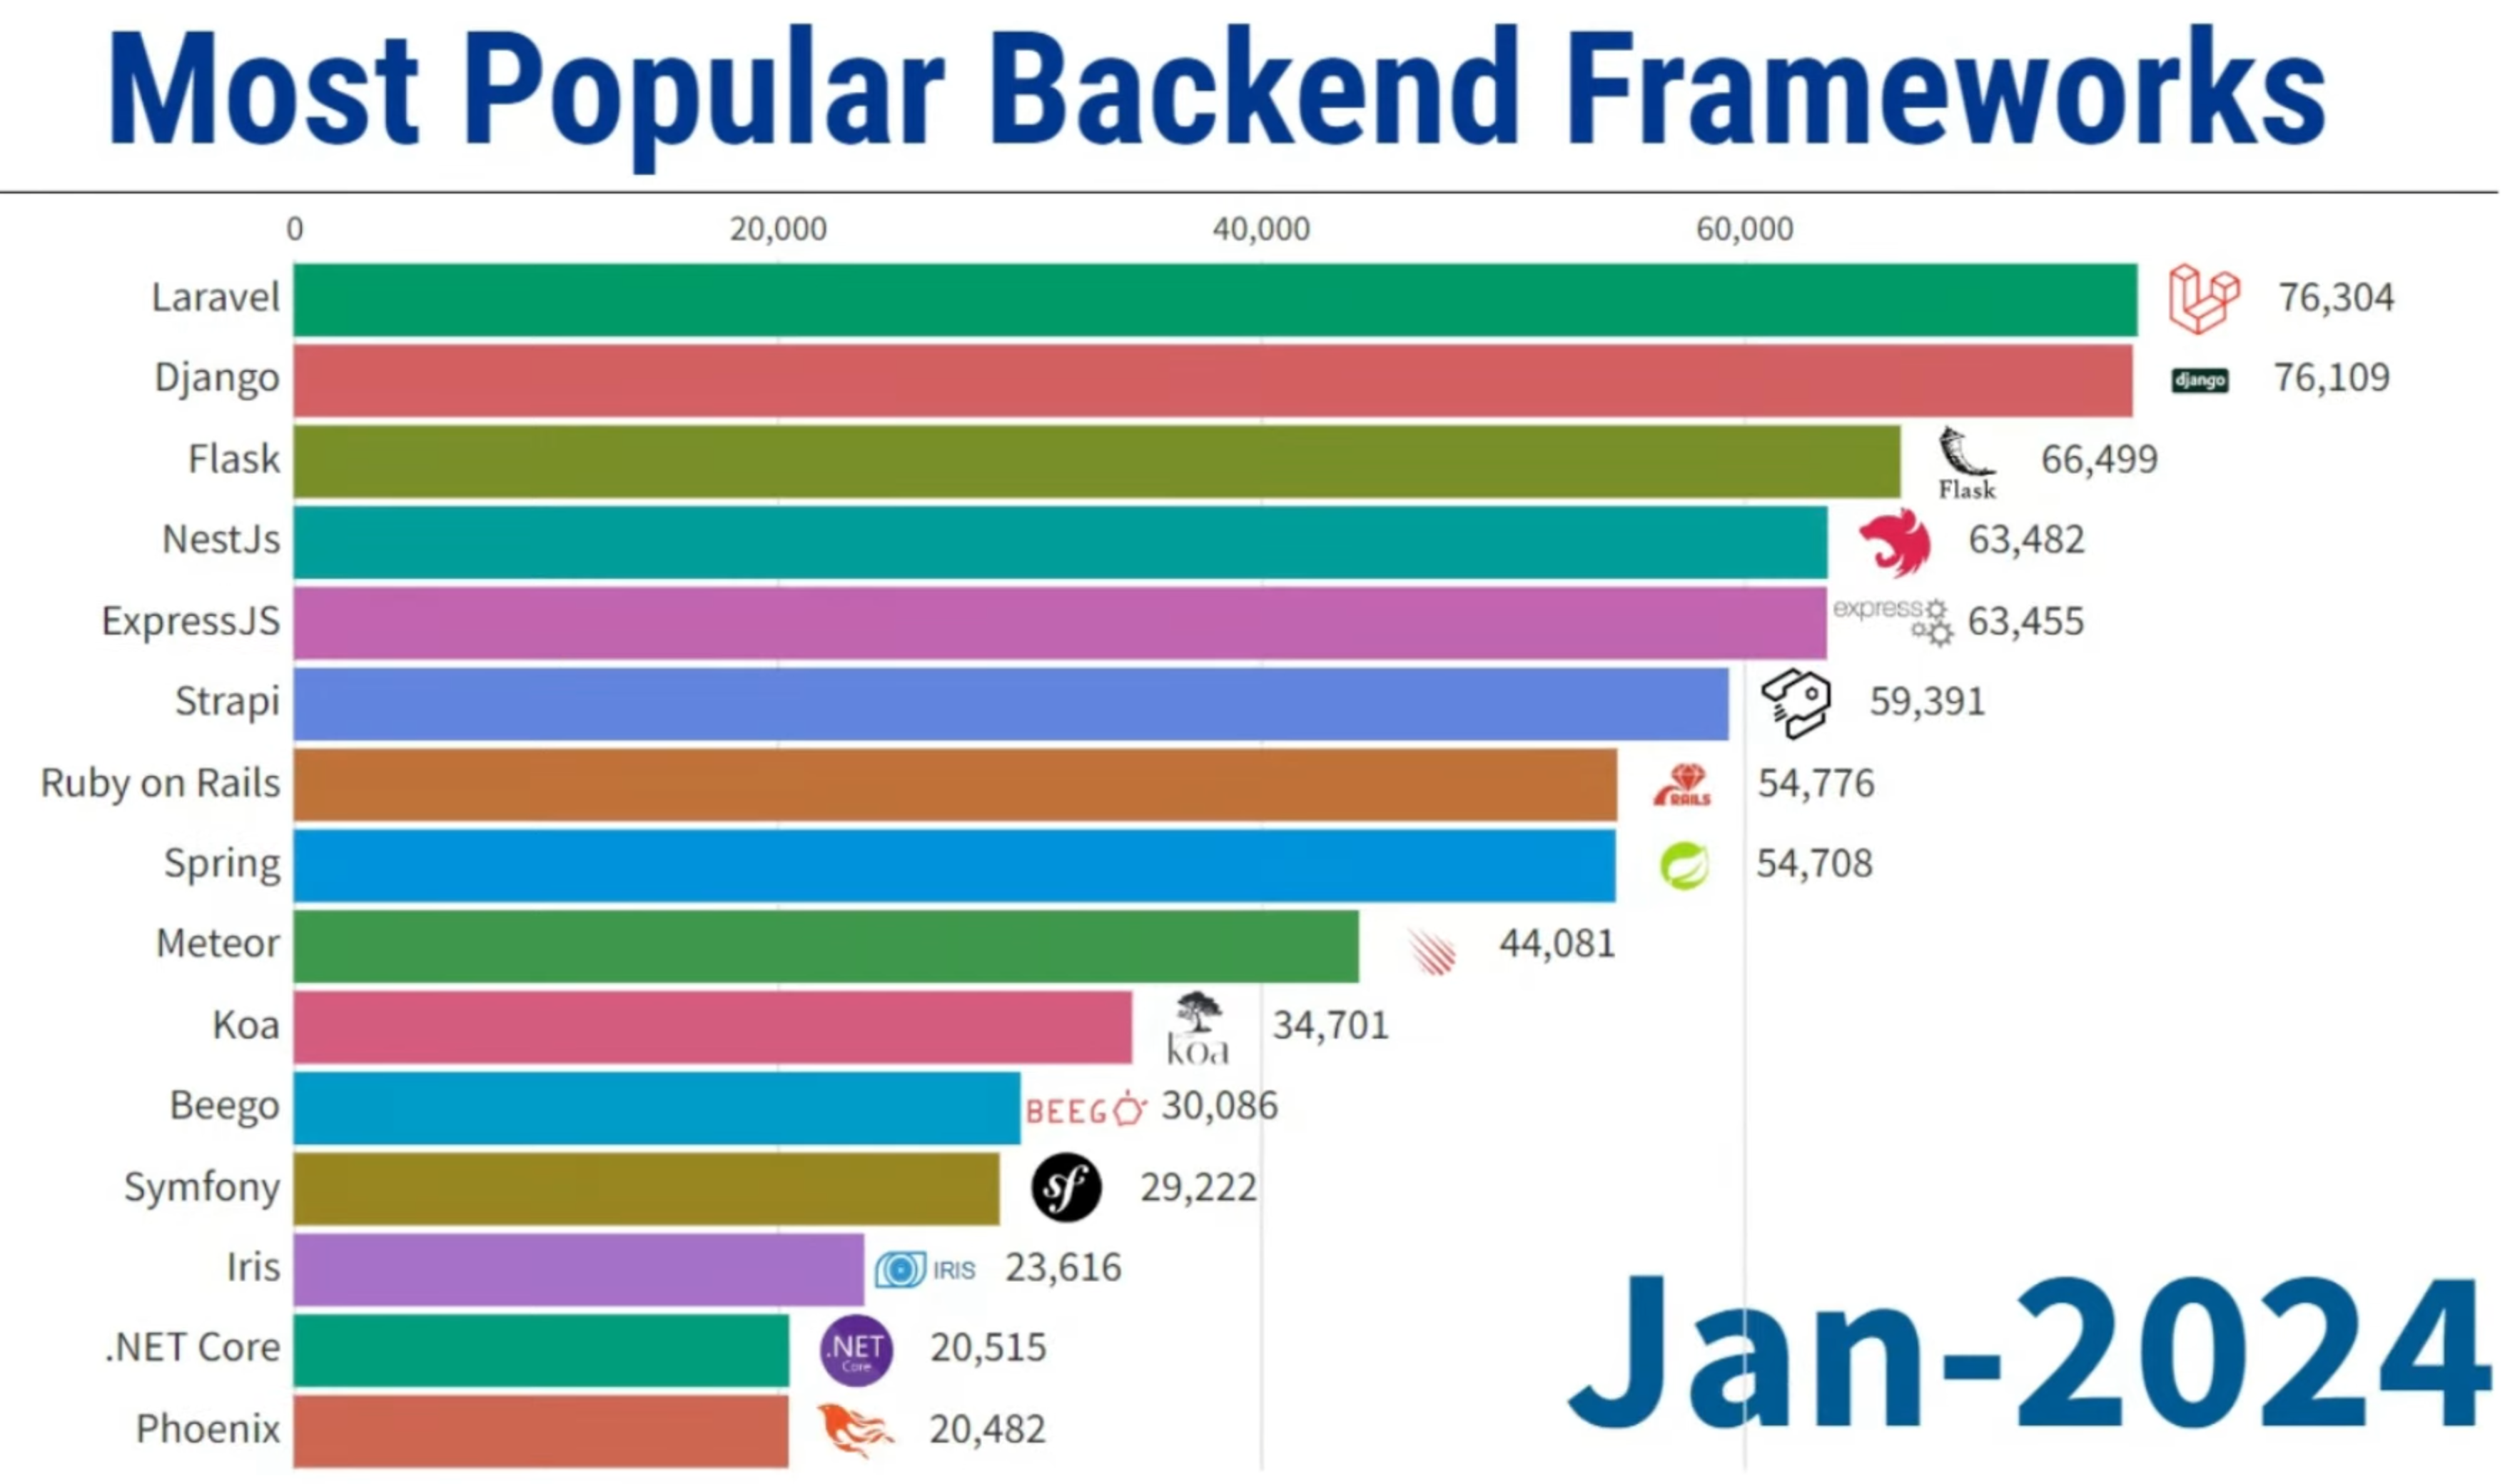
\includegraphics[width=0.95\textwidth]{gfx/figures/Popular_BE.png}
 \caption{Most Popular Backend Frameworks (Jan 2024) by GitHub Stars \cite{backend:popularity}}
 \label{fig:methodology:popularBE}
\end{figure}
~\\
The 15 most popular backend frameworks of January 2024 are displayed in \autoref{fig:methodology:popularBE}. The popularity for each framework of this list is calculated by the number of GitHub Stars from repositories listed in a GitHub Archive \cite{backend:popularity}. The selection options of the backend framework where based on this popularity list.

In addition to the previously stated criteria, the selected backend framework needed to meet specific performance requirements. It was essential for the framework to efficiently handle multiple connected clients with minimal latency. Furthermore, the framework's internal computation speed was critical, particularly for preparing input arguments for each task and managing task scheduling across all clients. The goal was to reduce overhead as much as possible to ensure high performance.
\begin{figure}[htbp]
  \myfloatalign
  \subfloat[Best fortunes responses per second (2023-10-17) \cite{backend:benchmark2}]{
    \label{fig:methodology:benchmark2BE}
    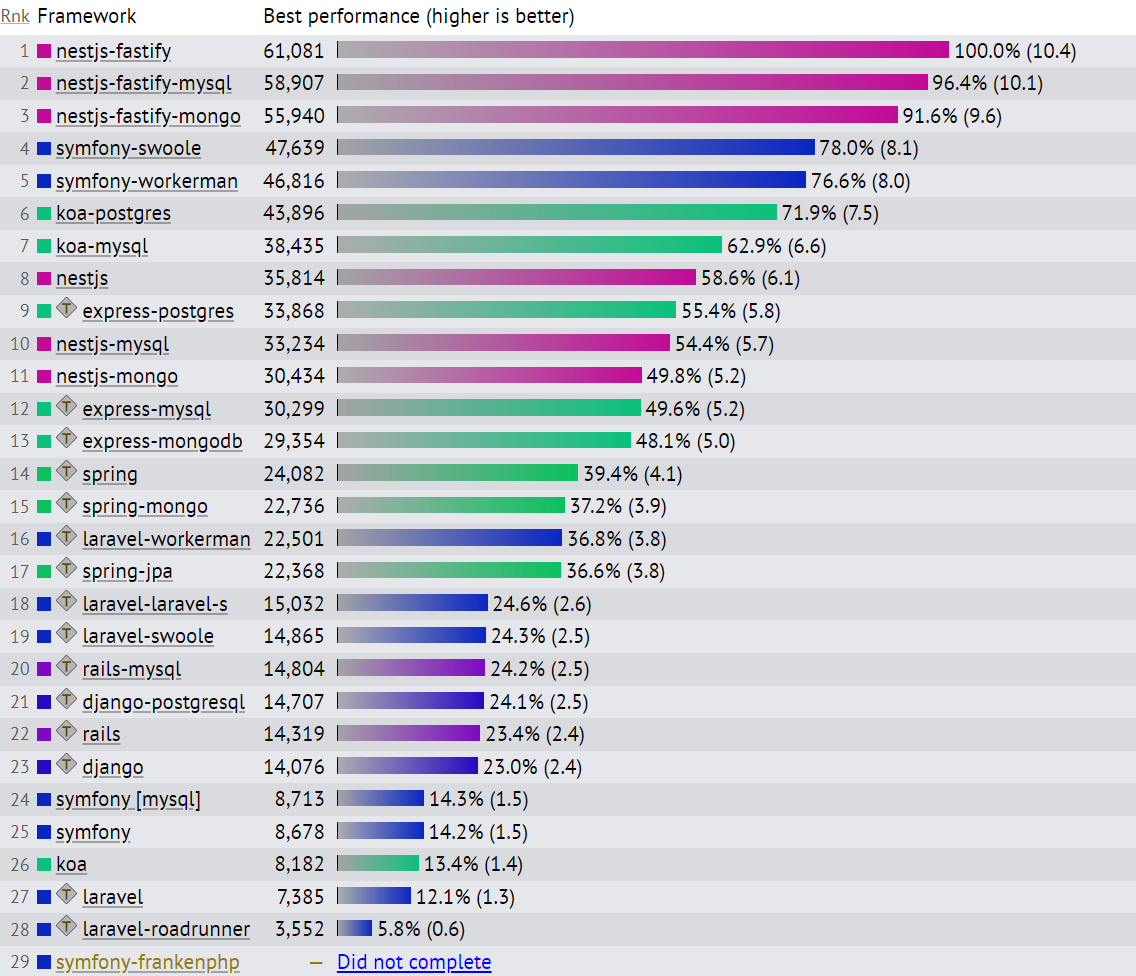
\includegraphics[width=.95\linewidth]{gfx/figures/Benchmark2_BE.png}
  }
  \caption{Most Popular Backend Frameworks from \autoref{fig:methodology:popularBE} Ranked by Performance.}
  \label{fig:methodology:benchmarkBE}
\end{figure}
\begin{figure}[htbp] \ContinuedFloat
  \myfloatalign
  \subfloat[Requests/Second (2024-06-25) \cite{backend:benchmark1}]{
     \label{fig:methodology:benchmark1BE}
     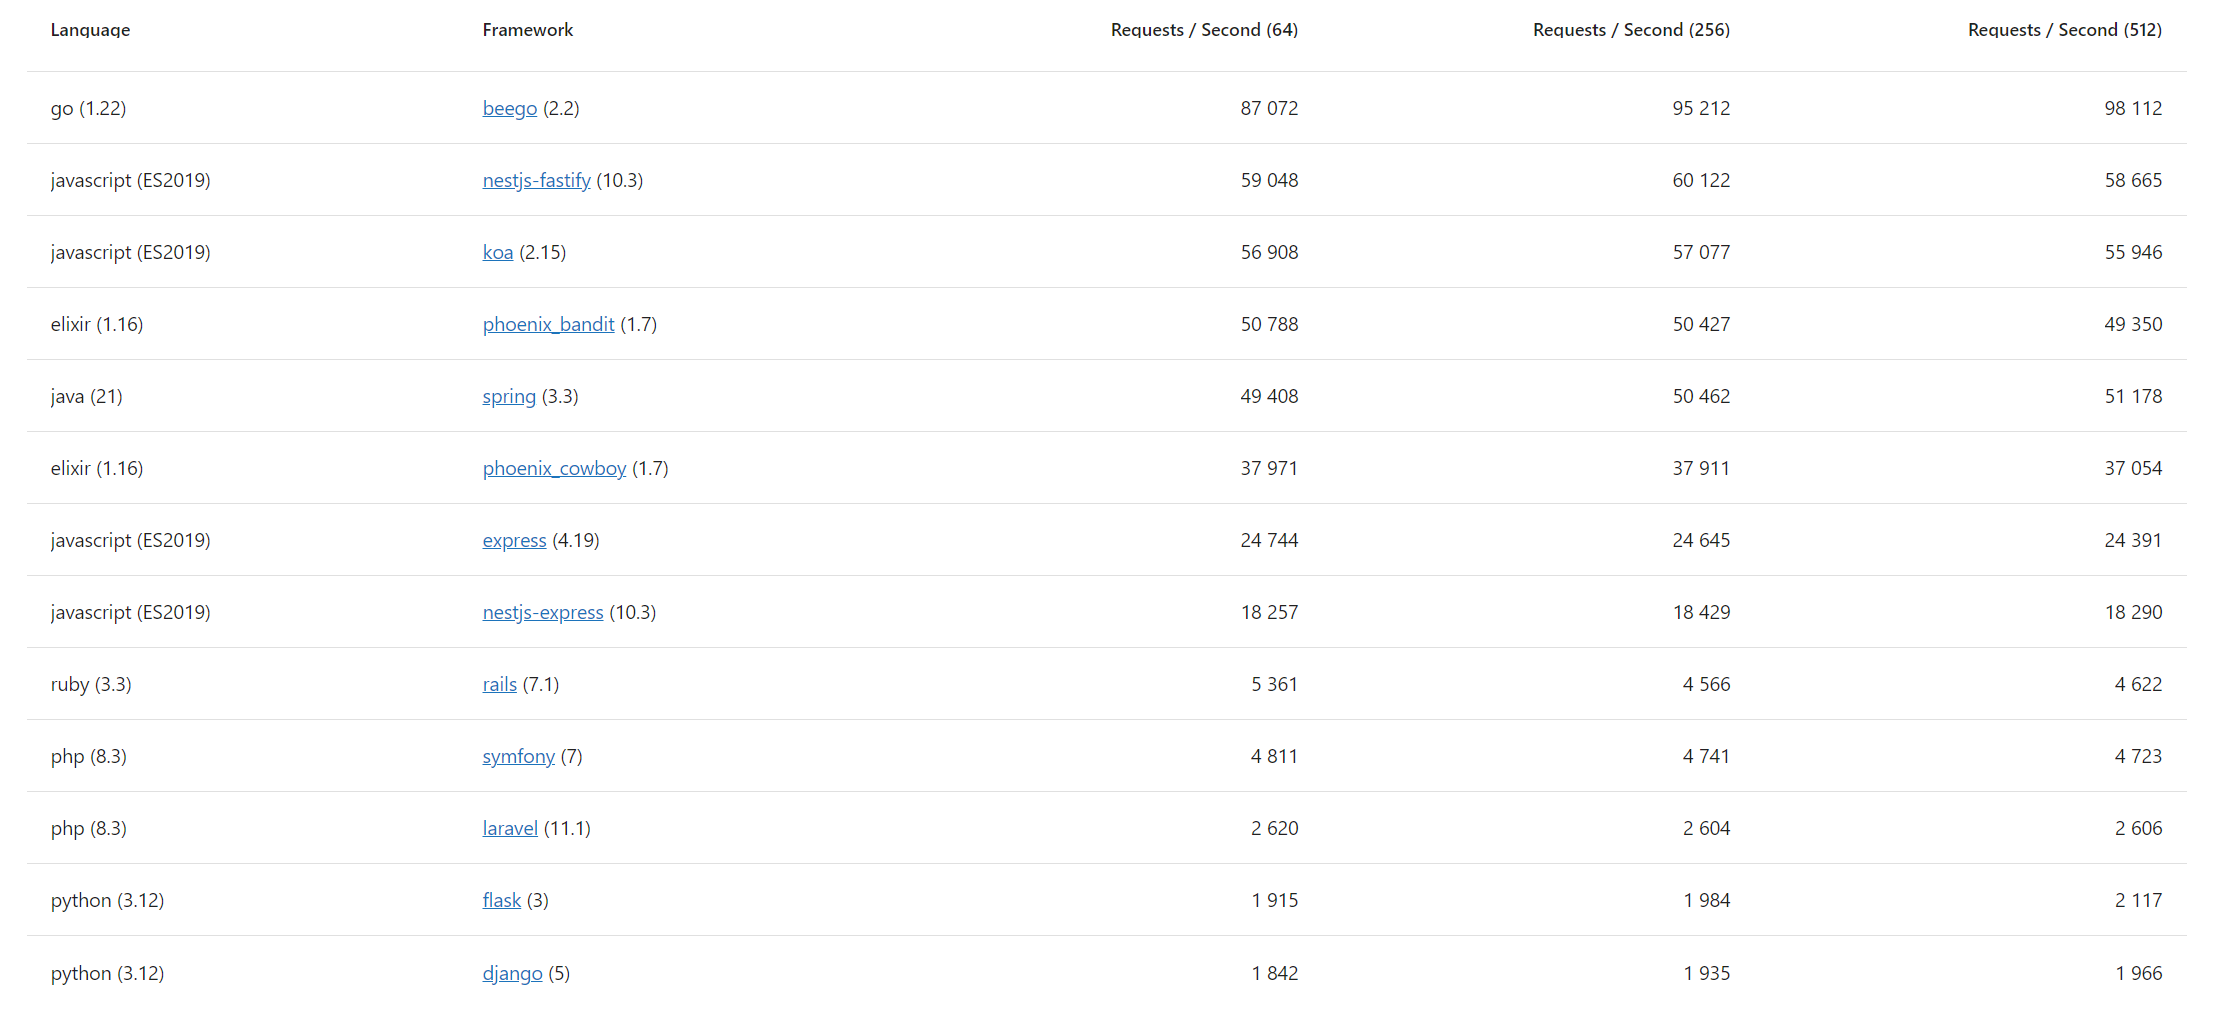
\includegraphics[width=.75\linewidth]{gfx/figures/Benchmark1_BE.png}
   }
   \caption{Most Popular Backend Frameworks from \autoref{fig:methodology:popularBE} Ranked by Performance.}
   \label{fig:methodology:benchmarkBE}
\end{figure}
~\\
To identify a high-performance framework, the most popular backend frameworks listed in \autoref{fig:methodology:popularBE} were compared by using two independent benchmark sources. The results of these benchmarks are presented in \autoref{fig:methodology:benchmarkBE}, where the frameworks are ranked from top to bottom based on their performance. It is important to note that some frameworks from the list in \autoref{fig:methodology:popularBE} where not part of these specific benchmarks. Both benchmark sources simulated numerous clients sending requests to each backend and measuring the number of successful responses per second in order to determine the performance \cite{backend:benchmark1, backend:benchmark2}.

Finally, NestJS \cite{methodology:nestjs} with Fastify was selected as the backend framework. It performed exceptionally well in both benchmarks shown in \autoref{fig:methodology:benchmarkBE} and is also a popular choice among developers.

\begin{figure}[htbp]
  \centering
  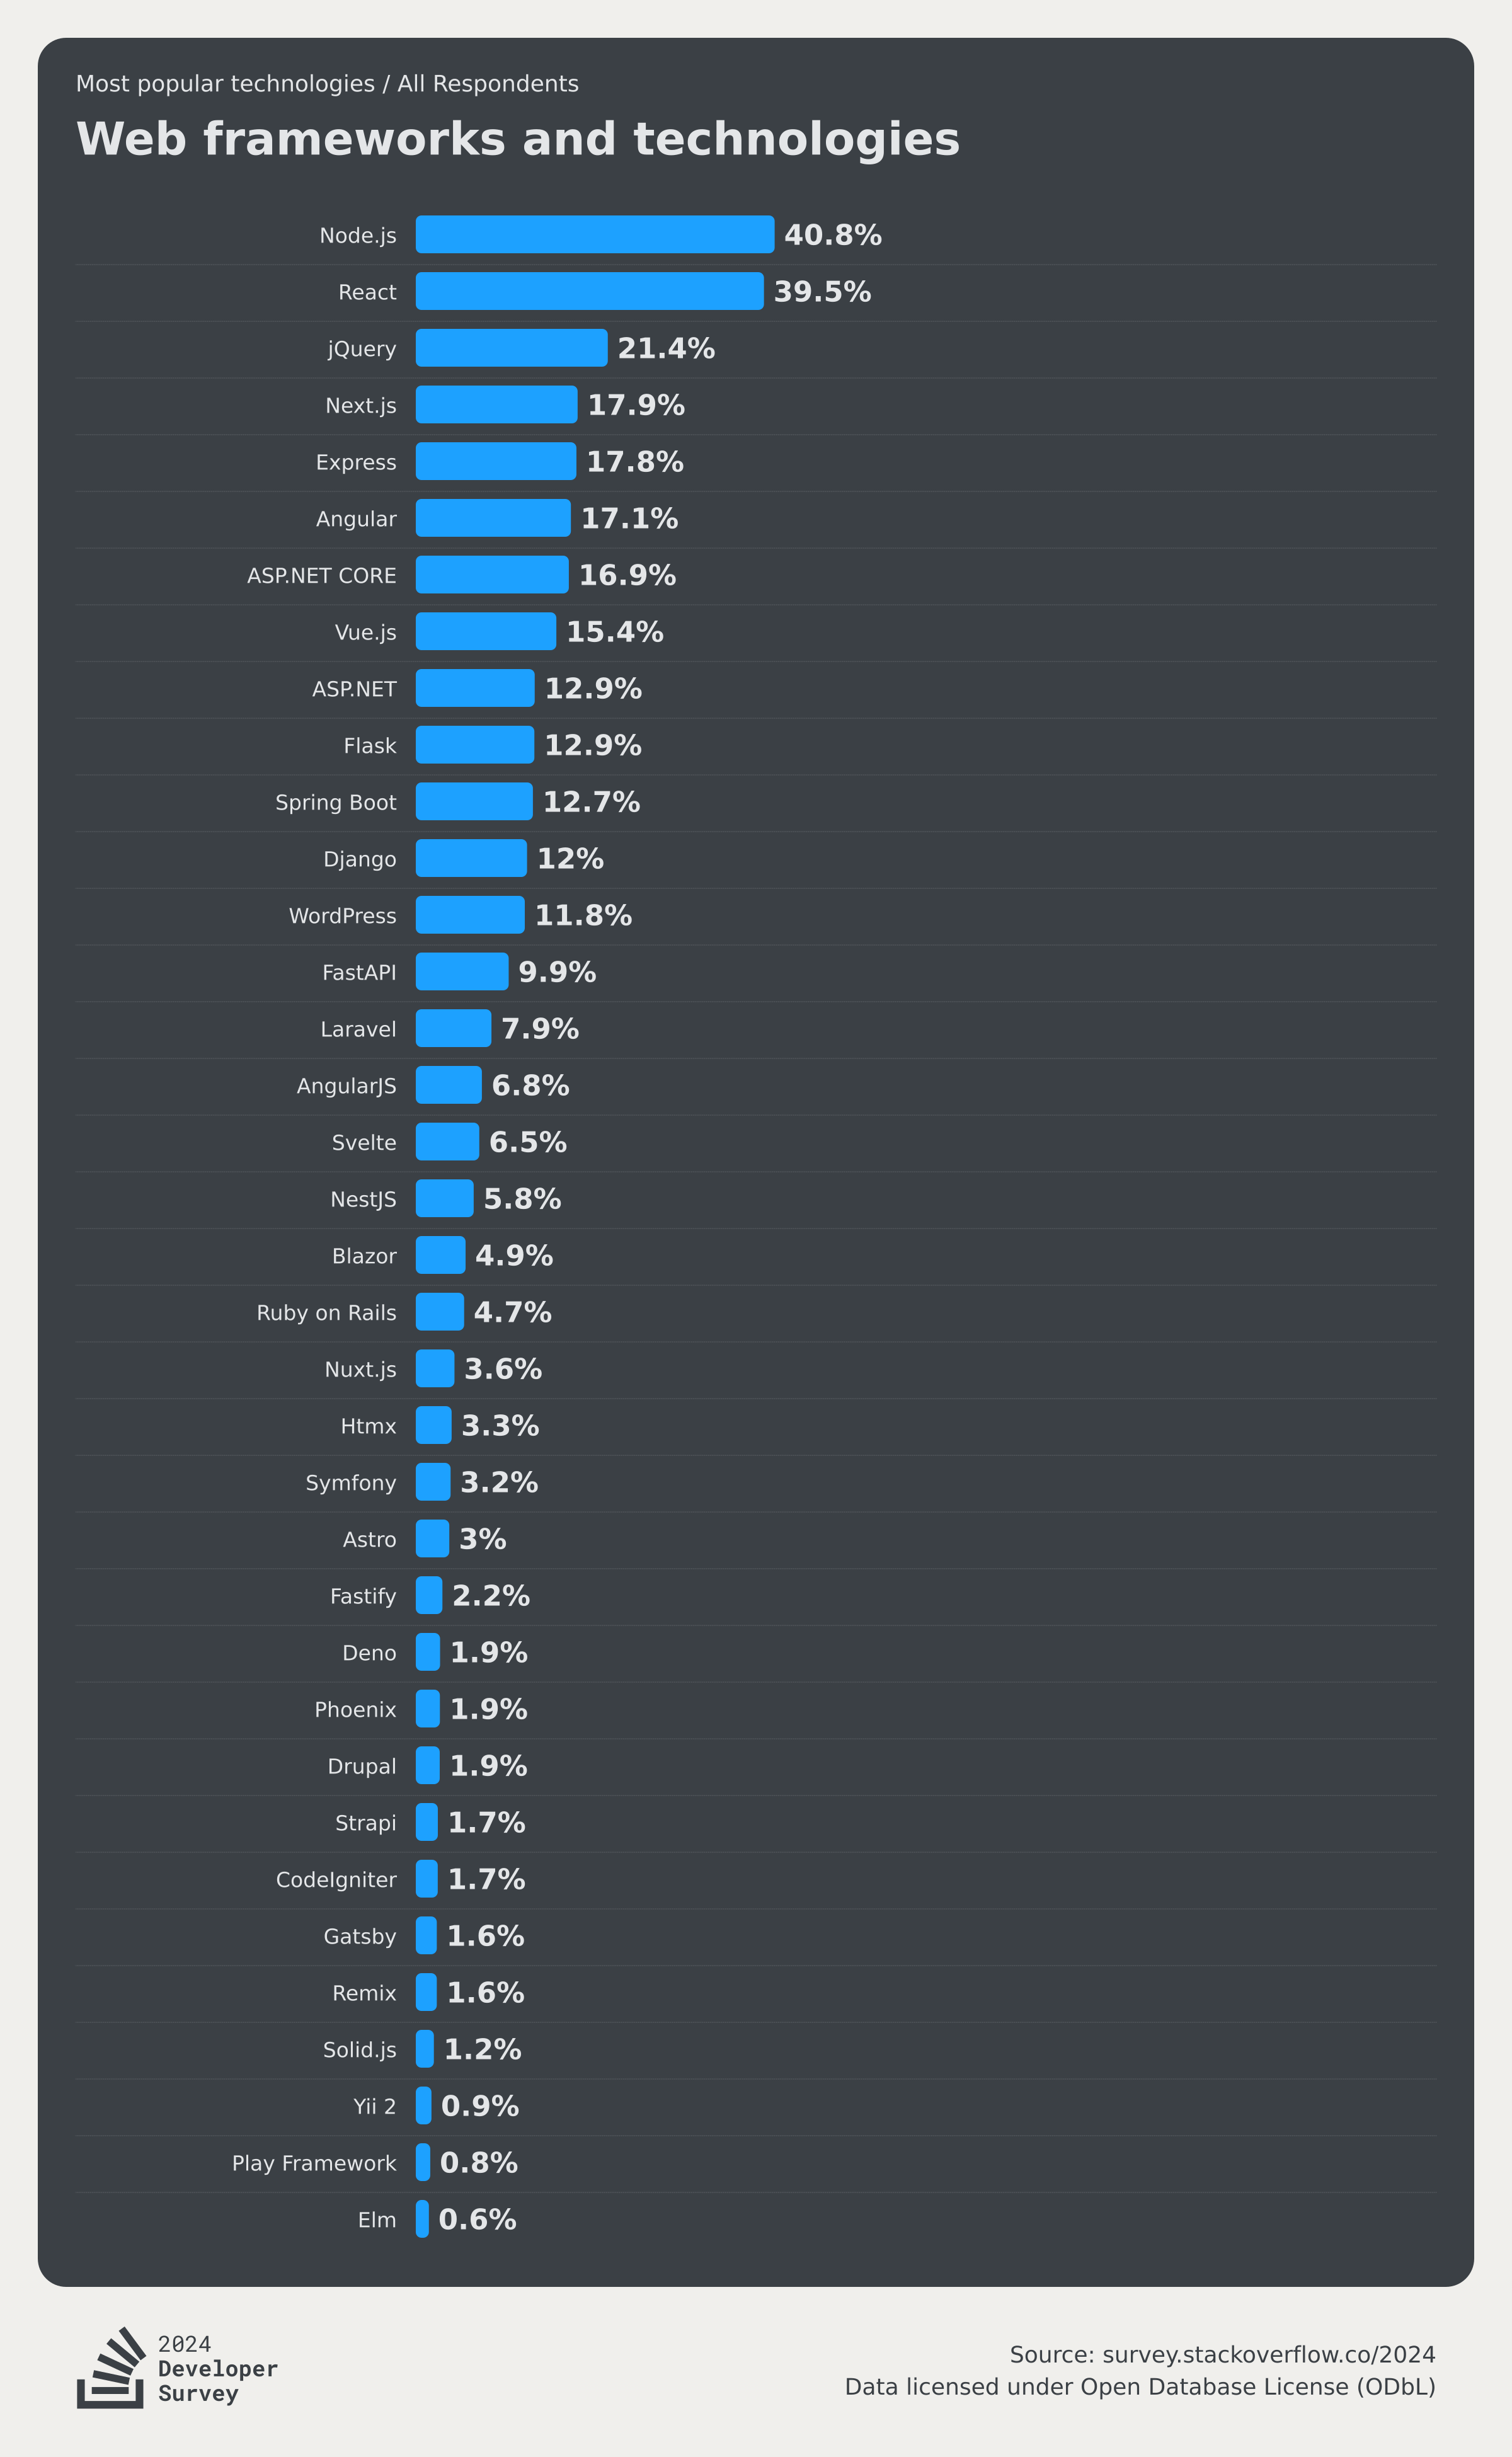
\includegraphics[width=0.95\textwidth]{gfx/figures/FrameworkSurvey2024.png}
  \caption{Most Used Web Frameworks and Technologies in 2024 (Developer Survey from Stack Overflow) \cite{frontend:popularity}}
  \label{fig:methodology:popularFE}
\end{figure}
\clearpage

\subsection{Frontend}
\label{subsec:methodology:frameworks:frontend}
The criteria stated in \autoref{sec:methodology:frameworks} also applied for the selection of a framework for the frontend. \autoref{fig:methodology:popularFE} shows the 36 most used frameworks among web developers in July 2024 \cite{frontend:popularity}. This statistic has been collected by Stack Overflow and is the result of a survey. In this survey web developers have been asked which web frameworks and web technologies they had been working with in the past year, and which do they want to work in over the next year \cite{frontend:popularity}. The two most popular options are, by far, Node.js and React with each around 40\% of votes. While Node.js is mainly used for backend development React is a JavaScript library used for frontend development. This is qualifying React as the choice of technology for the frontend development. Ranking fourth in \autoref{sec:methodology:frameworks} is Next.js with 17.9\% of votes. Next.js is a web framework based on React \cite{methodology:nextjs} and according to the survey the most popular React web framework in the year 2024. Therfore Next.js was selected as the framework for frontend development.

\section{WebAssembly}
\label{sec:methodology:wasm}
WebAssembly \cite{methodology:wasmW3C} is a key technology utilized in the implementation of WebArgo, offering several advantages for distributed or edge computing \cite{relatedwork:wasmedgecomputing}. It provides near-native performance, while maintaining platform independence \cite{methodology:wasm, methodology:wasmW3C, relatedwork:wasmedgecomputing}. 

WebAssembly is a low-level binary instruction format designed to serve as a compilation target for high-level programming languages \cite{methodology:wasm, methodology:wasmW3C, methodology:wasm2}, that promisses near-native performance execution in web browsers \cite{methodology:wasm, methodology:wasmW3C, relatedwork:wasmedgecomputing}. It employs a stack-based virtual machine architecture, operates in a memory-safe sandboxed environment, and interacts with JavaScript of the browser environment through a defined \ac{API} \cite{methodology:wasm, methodology:wasmW3C, methodology:wasm2, methodology:wasmdocu}. A compiled WebAssembly is particularly effective for computationally intensive tasks in the browser \cite{methodology:wasm2, methodology:wasmW3C} like image processing, game engines, or cryptographic operations.

The flexible features of platform independence and support of multiple high-level programming languages makes WebAssembly a fantastic choice for the WebArgo platfrom.
\\~\\
Furthermore, WebAssembly is maintaining the browsers inherent security model \cite{methodology:wasmW3C, methodology:wasm2, methodology:wasmdocu}. This is preventing any application to read and write files or to access device hardware such as cameras or microphones without explicit user permissions. Therfore WebArgo is ensuring a higher security for worker nodes than other volunteer computing applications, which require the installation of third-party software directly to the machine. This directly addresses the privacy and security concerns revealed by the study of \citeauthor{intro:volunteerStudy} \cite{intro:volunteerStudy} to increase the potential pool of participating workers.
\clearpage
\begin{figure}[htbp]
  \centering
  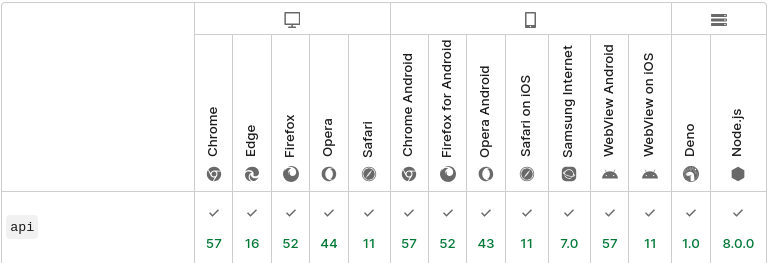
\includegraphics[width=0.95\textwidth]{gfx/figures/webassembly-browsercompability.png}
  \caption{Browser Compatibility: WebAssembly \cite{methodology:wasmdocu}}
  \label{fig:methodology:wasm}
\end{figure}
~\\
\autoref{fig:methodology:wasm} displays the browser compatibility of WebAssembly with multiple major browsers \cite{methodology:wasmdocu}. The check mark indicates WebAssembly support and the green number below marks the version since WebAssembly support was implemented. All browsers are sorted by desktop and mobile version. 

\subsection{emscriptren for C and C++}
\label{subsec:methodology:wasm:cpp}
The toolchain, used in this work, to compile C or C++ code into the WebAssembly binary format is emscripten. The team of emscripten already focused on the compilation of C and C++ code to \emph{asm.js} - a predecessor of WebAssembly - in the past \cite{methodology:emcc}. This compiler infrastructure has evolved to target the WebAssembly format, enabling the execution of native C/C++ applications in web browsers. Furthermore, emscripten provides the necessary JavaScript glue code to initialize the WebAssembly environment according to the compiled source code \cite{methodology:emcc}.

\subsection{Go}
\label{subsec:methodology:wasm:go}
The standard Go compiler inherently provides a option to directly target the WebAssembly format during the compilation process \cite{methodology:go}. This was utilized to support Go applications in WebArgo. Unlike emscripten, this compilation to WebAssembly is not producing a specific JavaScript glue code file for each Go application, however Go provides a general JavaScript glue code file suitable for all generated WebAssembly binaries \cite{methodology:go}. The files size of this general Go JavaScript glue code is surprisingly small compared to the JavaScript glue code generated by emscripten.

\subsection{Pyodie for Python}
\label{subsec:methodology:wasm:python}
Pyodide is described to be a port from CPython to WebAssembly/Emscripten \cite{methodology:pyodie}. It is a JavaScript library that provides a robust foreign function interface to compile python code to WebAssembly and execute it inside the browser environment \cite{methodology:pyodie}. Additionally it enables the installation and execution of Python packages inside the browser using micropip \cite{methodology:pyodie}. Also Pyodide promisses, that the executed Python code has full access to the Web \ac{API}s \cite{methodology:pyodie}, which is not an default feature of emscripten or Go.

Unfortunatly, Pyodide performed relatively slow compared to emscripten or Go during the testing of this work.

\section{WebSokets}
\label{sec:methodology:websokets}
WebSockets play a crucial role for the communication infrastructure of WebArgo. Different from standard \ac{HTTP} requests enable WebSockets a faster, bidirectional and full-duplex communication between clients and servers \cite{methodology:websockets1, methodology:websockets3, methodology:websockets2}. Unlike traditional \ac{HTTP} request-response patterns, WebSocket are establishing a persistent connections between client and server \cite{methodology:websockets3}, allowing real-time data transmission in both directions with minimal overhead after the initial handshake \cite{methodology:websockets3}. This protocol utilizes the ws:// or wss:// (secure) URI scheme and efficiently handles scenarios requiring live updates such as financial trading platforms, multiplayer games, or chat applications, with significantly reduced latency compared to polling mechanisms.

The real-time capability is leveraged for efficient task distribution, progress monitoring, and result collection in the implementation of the WebArgo platform. Additionally, is the bidirectional and full-duplex communication model extreamly usefull to handel the transmission of task and results between the server and workers. This replaces unperformant polling strategies and therfore enhances the performance of the communication process between server and workers.
\begin{figure}[htbp]
  \centering
  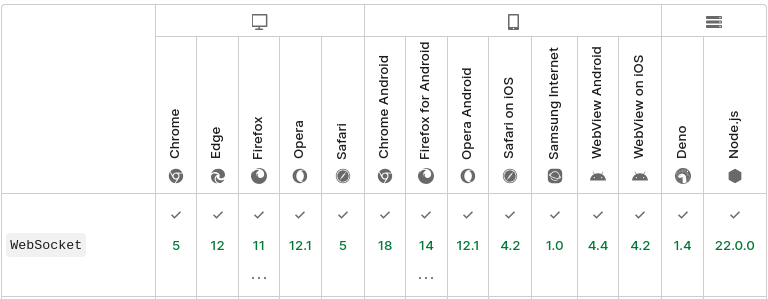
\includegraphics[width=0.95\textwidth]{gfx/figures/websocket-browsercompability.png}
  \caption{Browser Compatibility: WebSocket \cite{methodology:websockets1}}
  \label{fig:methodology:websocket}
\end{figure}
~\\
\autoref{fig:methodology:websocket} displays the browser compatibility of WebSocket with multiple major browsers \cite{methodology:websockets1}. The check mark indicates WebSocket support and the green number below marks the version since WebSocket support was implemented. All browsers are sorted by desktop and mobile version. 

\subsection{Socket.IO}
Socket.IO \cite{methodology:websockets2} is a popular JavaScript library that implements the usage of WebSockets on both the server and client side. NestJS \cite{methodology:nestjs}, the selected framework to implement the backend, has an inherent support of Socket.IO, using its concept of so called \emph{Gateways} \cite{methodology:nestjs}. Therfore the Socket.IO libary was selected to implement WebSocket inside the WebArgo platform.

\section{WebWorker}
\label{sec:methodology:webworker}
WebWorkers can be accessed through a specific JavaScript \ac{API}, enabling concurrent execution of scripts in background threads separate from the main browser UI thread \cite{methodology:webworkers}. These WebWorkers operate in an isolated context, communicating with the main thread through a message-passing interface, and therfore cannot directly access the \acs{HTML} \acs{DOM} of the web page \cite{methodology:webworkers}. 

This implementation of parallel processing through WebWorkers prevents the computationally intensive WebAssembly execution from blocking the user interface of a worker. This enables the worker to monitor the currently executed task and prevents an unpleasent user experience caused by an unexpectatly frozen screen. Furthermore, the WebWorker \ac{API} allows to create multiple WebWorkers in parallel. This feature could be used in the future to implement a browser based multi-threading solution for WebArgo.
\begin{figure}[htbp]
  \centering
  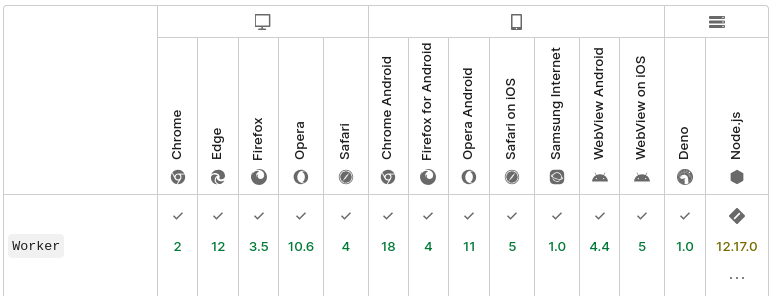
\includegraphics[width=0.95\textwidth]{gfx/figures/webworker-browsercompability.png}
  \caption{Browser Compatibility: WebWorker \cite{methodology:webworkers}}
  \label{fig:methodology:webworker}
\end{figure}
~\\
\autoref{fig:methodology:webworker} displays the browser compatibility of WebWorker with multiple major browsers \cite{methodology:webworkers}. The check mark indicates WebWorker support and the green number below marks the version since WebWorker support was implemented. All browsers are sorted by desktop and mobile version. 

\section{Benchmark: Visualizing the Mandelbrot set}
\label{sec:methodology:benchmark}
To benchmark the platform's performance, a computationally intensive job is implemented and executed across multiple connected workers. The total execution time is compared to the execution time of the same job on a single machine with native source code. The visualization of the Mandelbrot set represents all characteristics previously described in section \ref{sec:background:theory}, making it suitable as a job for this benchmark.

The Mandelbrot set is a famous subset of the complex numbers $\mathbb{C}$. \autoref{fig:methodology:mandelbrot} displays a coloriesed visualization of the set in the plane of complex numbers.
\begin{figure}[htbp]
  \centering
  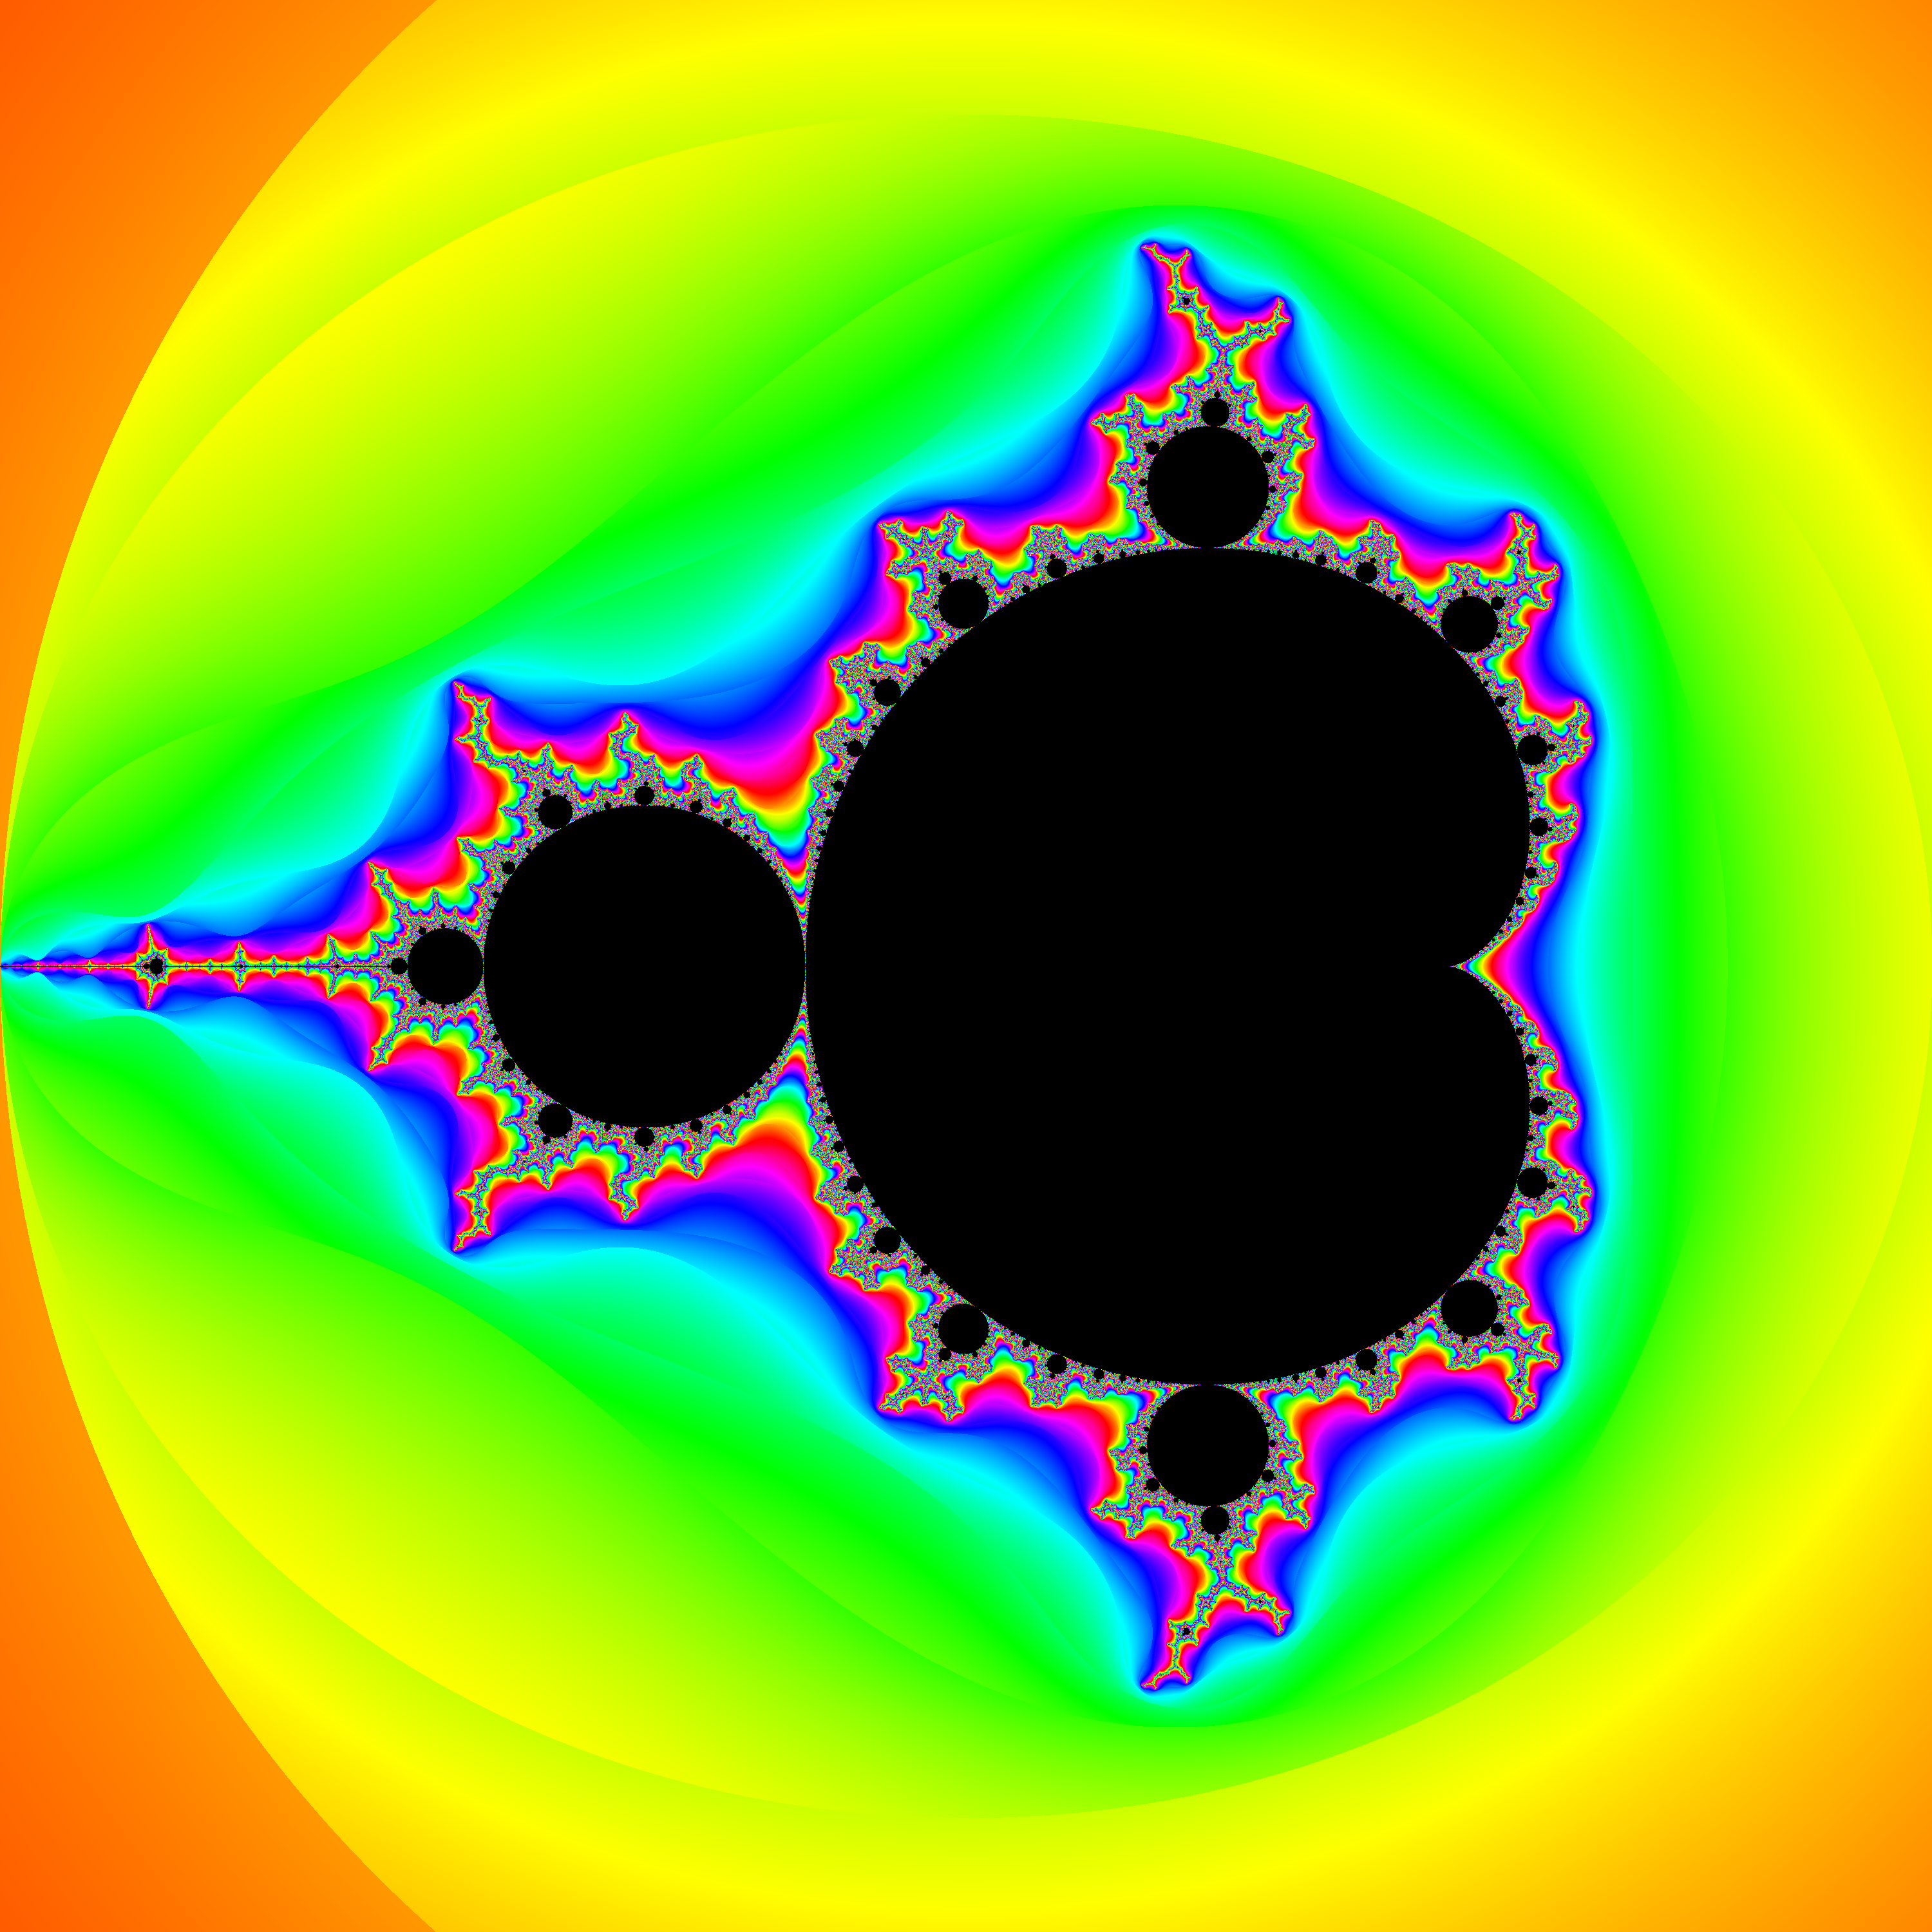
\includegraphics[width=0.95\textwidth]{gfx/figures/mandelbrot.png}
  \caption{Mandelbrot Set (Generated with Code in \autoref{app:code:mandelbrot1})}
  \label{fig:methodology:mandelbrot}
\end{figure}
~\\
To determine if a complex number $c$ is part of the Mandelbrot set, $c$ is applied to the function (\ref{equ:mandelbrot}) with $z_{0}=0$.
\begin{equation}
  z_{n+1} = z_{n}^2 + c
  \label{equ:mandelbrot}
\end{equation}
If the value of $z_{n+1}$ does not diverge over $n$ iterations, $c$ belongs to the Mandelbrot set. In \autoref{fig:methodology:mandelbrot}, all complex numbers $c$, for wich $z_{n+1}$ remains bounded over $n$ iterations are colored black. All other $c$ are colored based on the number of iterations required for $z_{n+1}$ to diverge, with the color spectrum ranging from red (low iteration count) over to blue (high iteration count) indicating increasing iteration counts.

The calculation and visualization of the Mandelbrot set can be partitioned into multiple tasks. Each task executes the same source code but with different input parameters, which define a unique two-dimensional area in the complex plane. These tasks can be executed in parallel due to the independence of calculations between different areas. The implementation for this benchmark is provided in \autoref{ch:appendix}. The source code for the native Go variant can be found in \autoref{app:code:mandelbrot1} and its Go-to-WebAssembly counterpart in \autoref{app:code:mandelbrot2}.